\input{../../preamble}

\title{Artificial Neural Networks}

\author{John Stachurski}


\date{2025}


\begin{document}

\begin{frame}
  \titlepage
\end{frame}



\begin{frame}
    \frametitle{Topics}

    \begin{itemize}
        \item Foo
        \vspace{0.5em}
        \item Bar
        \vspace{0.5em}
    \end{itemize}

\end{frame}


\begin{frame}{History}

    \begin{itemize}
        \item 1940s: \brown{McCulloch \& Pitts} create mathematical model of NN
        \vspace{0.5em}
        \item 1950s: \brown{Rosenblatt} develops the perceptron (trainable NN)
        \vspace{0.5em}
        \item 1960s-70s: Limited progress with single layer perceptrons
        \vspace{0.5em}
        \item 1980s: Backpropagation algorithm enables training of MLPs
        \vspace{0.5em}
        \item 1990s: SVMs temporarily overshadow ANNs in popularity
        \vspace{0.5em}
        \item 2000s: Deep learning finds successes in large problems
    \end{itemize}
    
        \vspace{0.5em}
        \vspace{0.5em}
    \emp{Last 10 years:} Explosion of progress in deep learning 

    \begin{itemize}
        \item CNNs, RNNs, LSTMs, transformers, LLMs, etc.
    \end{itemize}

\end{frame}

\begin{frame}{A model of the human brain}
    
    \begin{figure}
       \centering
       \scalebox{0.5}{\includegraphics[trim={0cm 0cm 0cm 0cm},clip]{brain.pdf}}
    \end{figure}

    \hspace{2em} -- source: Dartmouth undergraduate journal of science

\end{frame}


\begin{frame}{A mathematical representation: directed acyclic graph}
    
    \begin{figure}
       \centering
       \scalebox{0.24}{\includegraphics[trim={0cm 0cm 0cm 0cm},clip]{graph.pdf}}
    \end{figure}

\end{frame}

\begin{frame}
    
    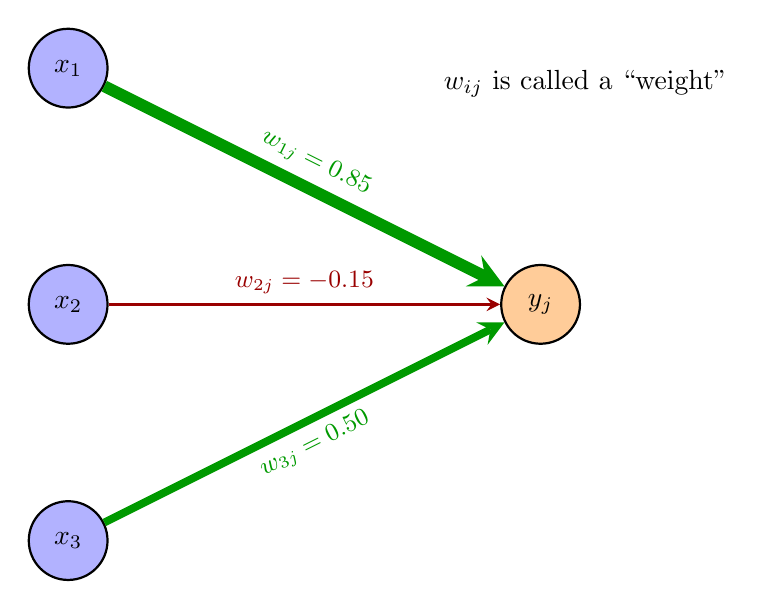
\begin{tikzpicture}[
            neuron/.style={circle, draw=black, fill=white, minimum size=1cm, thick},
            input neuron/.style={neuron, fill=blue!30},
            output neuron/.style={neuron, fill=orange!40},
            strong pos/.style={green!60!black, line width=1.5mm, ->, >=stealth},
            medium pos/.style={green!60!black, line width=1mm, ->, >=stealth},
            weak neg/.style={red!60!black, line width=0.4mm, ->, >=stealth},
            label/.style={font=\small}
        ]

        % Input neurons (left column)
        \node[input neuron] (N1) at (0,3) {$x_1$};
        \node[input neuron] (N2) at (0,0) {$x_2$};
        \node[input neuron] (N3) at (0,-3) {$x_3$};

        % Output neuron (right column)
        \node[output neuron] (N4) at (6,0) {$y_j$};

        
        \node[anchor=south east, font=\normalsize] at (8.5, 2.5) {$w_{ij}$ is called a ``weight''};

        % Connections with weights
        \draw[strong pos] (N1) -- node[label, above, sloped] {$w_{1j} = 0.85$} (N4);
        \draw[weak neg] (N2) -- node[label, above] {$w_{2j} = -0.15$} (N4);
        \draw[medium pos] (N3) -- node[label, below, sloped] {$w_{3j} = 0.50$} (N4);

    \end{tikzpicture}

\end{frame}

\begin{frame}
    
    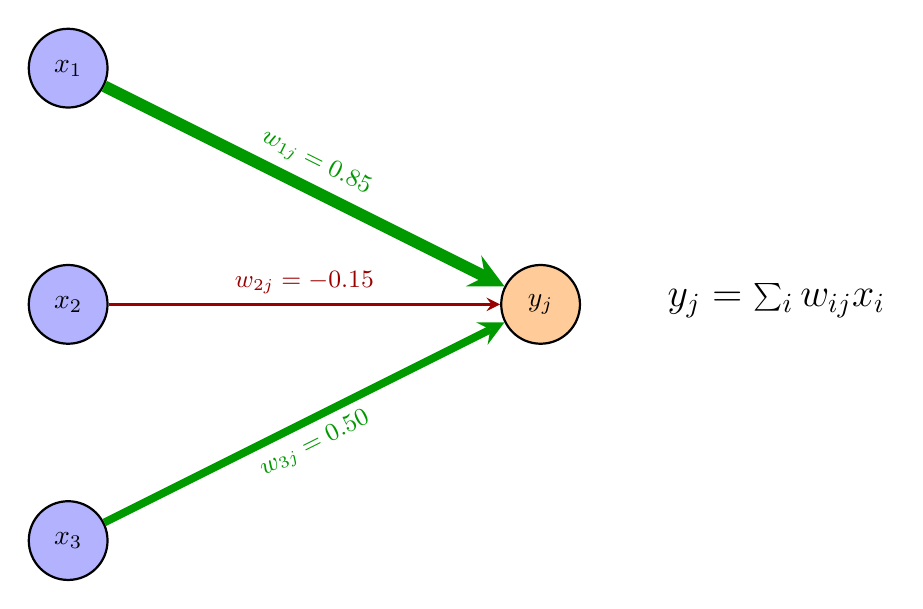
\begin{tikzpicture}[
            neuron/.style={circle, draw=black, fill=white, minimum size=1cm, thick},
            input neuron/.style={neuron, fill=blue!30},
            output neuron/.style={neuron, fill=orange!40},
            strong pos/.style={green!60!black, line width=1.5mm, ->, >=stealth},
            medium pos/.style={green!60!black, line width=1mm, ->, >=stealth},
            weak neg/.style={red!60!black, line width=0.4mm, ->, >=stealth},
            label/.style={font=\small}
        ]

        % Input neurons (left column)
        \node[input neuron] (N1) at (0,3) {$x_1$};
        \node[input neuron] (N2) at (0,0) {$x_2$};
        \node[input neuron] (N3) at (0,-3) {$x_3$};

        % Output neuron (right column)
        \node[output neuron] (N4) at (6,0) {$y_j$};

        
        \node[anchor=south east, font=\Large] at (10.5, -0.3)
            {$y_j = \sum_i w_{ij} x_i$};

        % Connections with weights
        \draw[strong pos] (N1) -- node[label, above, sloped] {$w_{1j} = 0.85$} (N4);
        \draw[weak neg] (N2) -- node[label, above] {$w_{2j} = -0.15$} (N4);
        \draw[medium pos] (N3) -- node[label, below, sloped] {$w_{3j} = 0.50$} (N4);

    \end{tikzpicture}

\end{frame}

\begin{frame}
    
    % Neural Network with 3 input neurons and 2 output neurons
% To be included in an existing LaTeX document
% Required packages: tikz

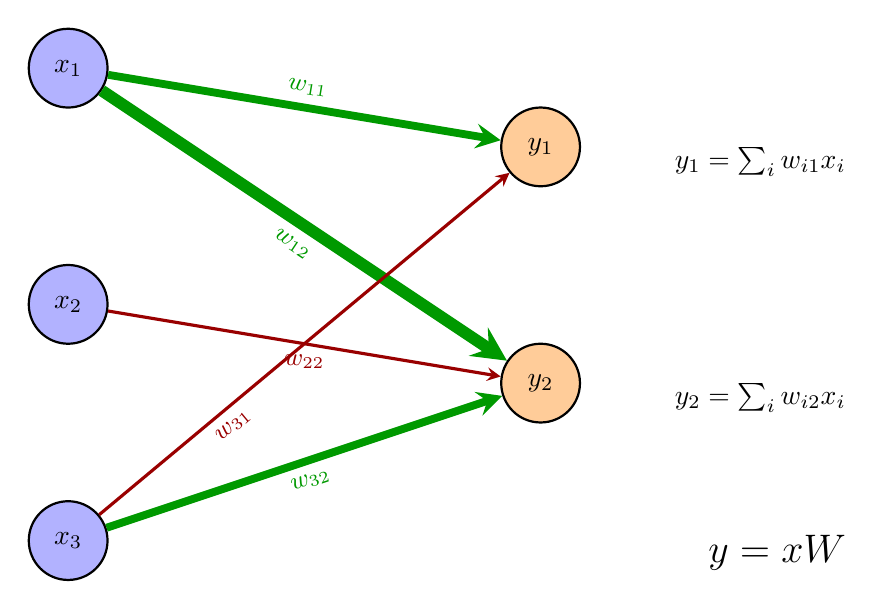
\begin{tikzpicture}[
        neuron/.style={circle, draw=black, fill=white, minimum size=1cm, thick},
        input neuron/.style={neuron, fill=blue!30},
        output neuron/.style={neuron, fill=orange!40},
        strong pos/.style={green!60!black, line width=1.5mm, ->, >=stealth},
        medium pos/.style={green!60!black, line width=1mm, ->, >=stealth},
        weak neg/.style={red!60!black, line width=0.4mm, ->, >=stealth},
        label/.style={font=\small}
    ]

    % Input neurons (left column)
    \node[input neuron] (N1) at (0,3) {$x_1$};
    \node[input neuron] (N2) at (0,0) {$x_2$};
    \node[input neuron] (N3) at (0,-3) {$x_3$};

    % Output neurons (right column)
    \node[output neuron] (N5) at (6,2) {$y_1$};
    \node[output neuron] (N4) at (6,-1) {$y_2$};

    % Connections with weights to N4
    \draw[strong pos] (N1) -- node[label, below, sloped] {$w_{12}$} (N4);
    \draw[weak neg] (N2) -- node[label, below] {$w_{22}$} (N4);
    \draw[medium pos] (N3) -- node[label, below, sloped] {$w_{32}$} (N4);

    % Some connections to the new neuron N5
    \draw[medium pos] (N1) -- node[label, above, sloped] {$w_{11}$} (N5);
    \draw[weak neg] (N3) -- node[label, below, sloped, pos=0.3] {$w_{31}$} (N5);

    % Text in bottom right
    \node[anchor=south east, font=\normalsize] at (10, 1.5) {$y_1 = \sum_i w_{i1} x_i$};
    \node[anchor=south east, font=\normalsize] at (10,-1.5) {$y_2 = \sum_i w_{i2} x_i$};
    \node[anchor=south east, font=\Large] at (10,-3.5) {$\implies y = x W$};

\end{tikzpicture}

\end{frame}


\begin{frame}
    
    In fact we add a bias term as well

    \begin{equation*}
        y_j = \sum_i w_{ij} x_i       
        \qquad \to \qquad
        y_j = \sum_i w_{ij} x_i + b_j
    \end{equation*}

    And also a nonlinear ``activation function'' $\sigma \colon \RR \to \RR$
    %
    \begin{equation*}
        y_j = \sum_i w_{ij} x_i + b_j
        \qquad \to \qquad
        y_j = \sigma \left(\sum_i w_{ij} x_i + b_j \right)
    \end{equation*}

    Applying $\sigma$ pointwise, we can write this in vector form as
    %
    \begin{itemize}
        \item $y = \sigma(x W + b)$ or
        \item $y = \sigma(Ax)$  where $Ax = xW + b$
    \end{itemize}

    
\end{frame}

\begin{frame}{Common activation functions}
    
    \begin{figure}
       \centering
       \scalebox{0.54}{\includegraphics[trim={0cm 0cm 0cm 0cm},clip]{activations.pdf}}
    \end{figure}


\end{frame}

\begin{frame}
    
    Aim: approximate an unknown functional relationship
    %
    \begin{equation*}
        y = f(x)
        \qquad (x \in \RR^k, \; y \in \RR)
    \end{equation*}

    \Egs
    %
    \begin{itemize}
        \item $x = $ cross section of returns, $y = $ return on oil futures tomorrow
        \vspace{0.5em}
        \item $x = $ weather sensor data, $y = $ max temp tomorrow
    \end{itemize}
        \vspace{0.5em}
        \vspace{0.5em}

    Problem:

    \begin{itemize}
        \item observe $(x_i, y_i)_{i=1}^n$ and seek $f$ such that $y_{n+1}
            \approx f(x_{n+1})$
    \end{itemize}


\end{frame}



\begin{frame}

    Nonlinear regression: choose model $\{f_\theta\}_{\theta \in \Theta}$ and minimize the empirical loss
    %
    \begin{equation*}
        \ell(\theta) := \frac{1}{n}\sum_{i=1}^n (y_i - f_\theta(x_i))^2
        \quad \st \quad \theta \in \Theta
    \end{equation*}


    \pause
    \vspace{0.5em}
    In the case of ANNs, we consider all $f_\theta$ having the form
    %
    \begin{equation*}
        f_\theta
        = \sigma \circ A_{m} 
            \circ \cdots \circ \sigma \circ A_{2}  \circ \sigma \circ A_{1}
    \end{equation*}
    %
    where
    %
    \begin{itemize}
        \item $A_{\ell} x = x W_\ell + b_\ell $ is an affine map 
        \vspace{0.5em}
        \item $\sigma$ is a nonlinear ``activation'' function
    \end{itemize}

\end{frame}

\begin{frame}

    Minimizing the loss functions  
    
    \begin{figure}
       \begin{center}
        \scalebox{0.15}{\includegraphics[trim={0cm 0cm 0cm 0cm},clip]{gdi.png}}
       \end{center}
    \end{figure}

    Source: \url{https://danielkhv.com/}

\end{frame}


\begin{frame}{Gradient descent}

    Algorithm:
    
    \begin{equation*}
        \theta_{\rm{next}} = \theta - \lambda \, \nabla_\theta \ell(\theta, x, y)
    \end{equation*}

    \begin{itemize}
        \item take a step in the opposite direction to the grad vector
        \vspace{0.5em}
        \item $\lambda$ is the \emp{learning rate} -- often changes at each step
        \vspace{0.5em}
        \item iterate until hit a stopping condition
        \vspace{0.5em}
        \item in practice replace $\ell(\theta)$ with batched loss
            %
            \begin{equation*}
                \frac{1}{|B|}\sum_{i \in B} (y_i - f_\theta(x_i))^2
            \end{equation*}
    \end{itemize}

    Using batches $\to$ \emp{stochastic gradient descent}

\end{frame}


\begin{frame}{Extensions}

    Different loss functions, different architectures

    \begin{itemize}
        \item Loss functions with regularization
        \vspace{0.5em}
        \item -- insert other loss funcs --
        \vspace{0.5em}
        \item Convolutional neural networks
        \vspace{0.5em}
        \item Recurrent neural networks
        \vspace{0.5em}
        \item Transformers, etc.
    \end{itemize}
    
\end{frame}



\begin{frame}
    
    Why is deep learning so successful for some problems?

    Story 1 -- human brain, universal function approx, can break curse of dim

    Story 2 -- a flexible function fitting technique that extends well to high
        dimensions and has received massive investment from the CS community

\end{frame}

\end{document}


